\documentclass[10pt,a4paper]{article}
\usepackage[utf8]{inputenc}
\usepackage[german]{babel}
\usepackage[T1]{fontenc}
\usepackage{amsmath}
\usepackage{amsfonts}
\usepackage{amssymb}
\usepackage{float}
\usepackage{graphicx}
\renewcommand\thesubsection{\alph{subsection}}
\begin{document}

\begin{center}
Modellierung Phyiskalischer Systeme: Praktikum 1

Johannes Reidl, Sigurd Sippel

\end{center}

\section{Weltraummission}

\subsection{Satellitensimulation Erdumkreisung, Fluggeschwindigkeit, geostationäre Bahn}

Das Schaltbild für die Simulation eines Satelliten um die Erde, enthält die Startparameter Startflugwinkel $\theta$, Starthöhe $h_0$, Startgeschwindigkeit $v_0$ und Startpositionswinkel $\delta$.  Es wir die Position ($x_{sat}$,$y_{sat}$  des Satelliten berechnet.

	\begin{figure}[H]
		\centering
		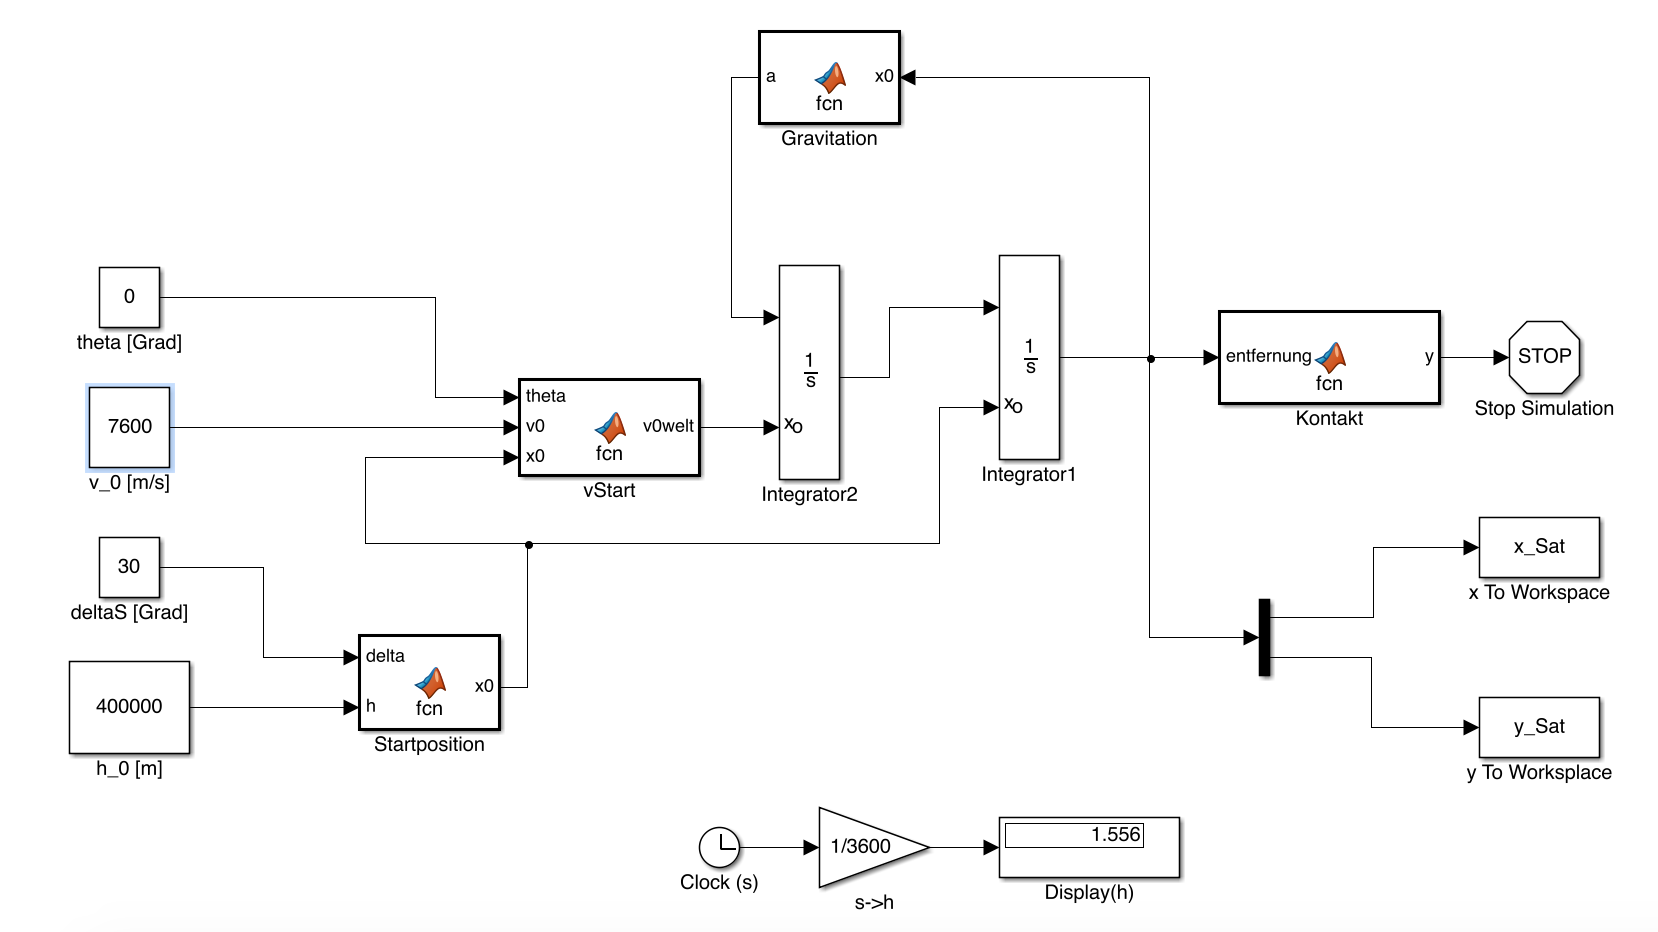
\includegraphics[width=1\textwidth]{../aufgabe1/screens/simulink.png}
		\caption{Schaltbild Erdumkreisung des Satelliten}
	\end{figure}

Berechnung der Startposition:

\begin{align}
function \: x0 = start(delta, h) 
\\er = 6378000; \nonumber %Erdradius in Meter
\\bogen_\delta = delta * pi / 180;\nonumber
\\x  = cos(bogen_{\delta}) * (er + h); \nonumber
\\y  = sin(bogen_{\delta}) * (er + h);\nonumber
\\ x0 = [x ; y]\nonumber
\end{align}

Berechnung des Geschwindigkeitsvektors:

\begin{align}
function \: v0welt = vStart(theta, v_0, x_0)
\\bogen_\theta = \theta * pi / 180; \nonumber
\\norm_E = x_0 / norm(x_0);   \nonumber           % Einheitsvektor in Normalrichtung
\\tan_E = [normE(2) ; -normE(1)];  \nonumber    % Einheitsvektor in Tangentialrichtung (90 Grad gedreht)
\\t = cos(bogen_{\theta}) * v_0;  \nonumber        % Tangentialkomponente
\\n = sin(bogen_{\theta}) * v_0;   \nonumber       % Normalkomponente
\\v0welt = (t * tan_E) + (n * norm_E);  \nonumber % Geschwindigkeitsvektor
\end{align}
	
Berechnung der Gravitation:

\begin{align}
function a = Gravitation(x_0)
\\G = 66.7 * 10^(-12);  \nonumber % Gravitationskonstante 
\\m_{Erde} = 5.9 * 10^24;  \nonumber % Masse der Erde 
\\r_{Erde} = norm(x_0);  \nonumber % Entfernung zur Erde 
\\richtung = -x0 / r_{Erde}; \nonumber
\\a = richtung * (G * m_{Erde} /(r_{Erde})^2) \nonumber % Gravitationsbeschleunigung: a = m * G / r^2 
\end{align}

Berechnung des Ereignisses 'Kontakt zur Erde':

\begin{align}
function y = Kontakt(entfernung)
\\entfernung = norm(entfernung); \nonumber
\\if(entfernung<=6378000) \:
    y = 1; \nonumber
\\else \: \nonumber
    y = 0; 
\\end; \nonumber
\end{align}


\subsubsection{Erdumkreisung}
Bei einer Startgeschwindigkeit $v0 = 7600 m/s$ und einer Simulationszeit von $5600s = 1.556 h$ ergibt sich folgende Umlaufbahn
Sim time = 5600 s = 1.556 h
	\begin{figure}[H]
		\centering
		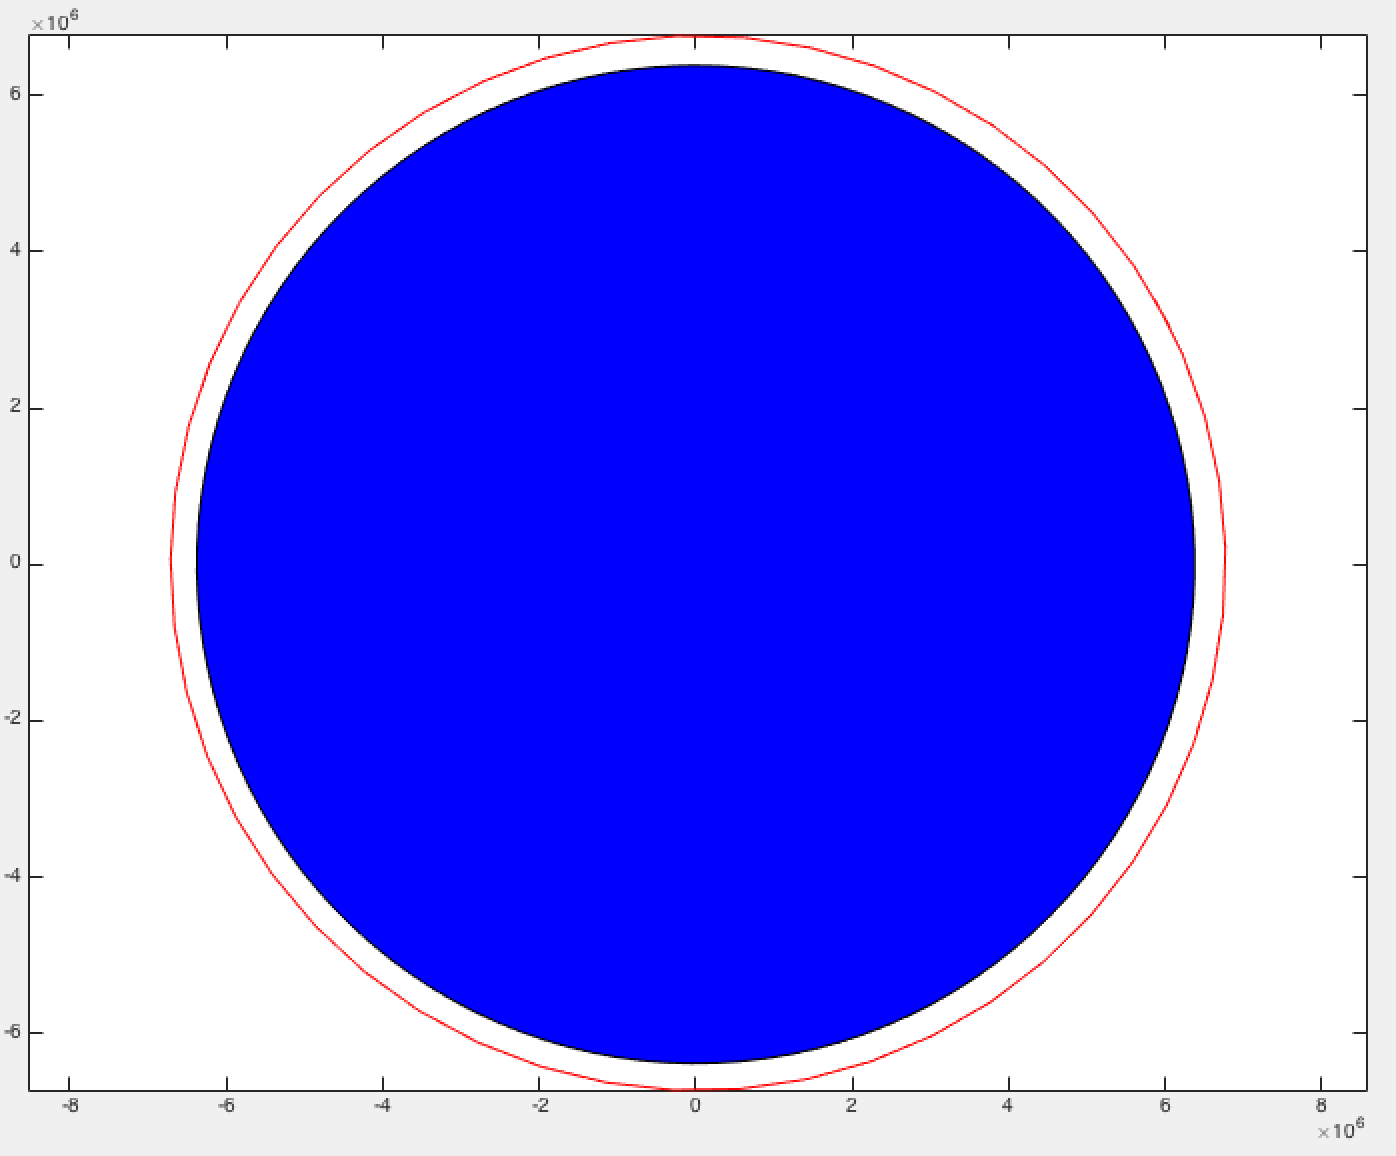
\includegraphics[width=0.5\textwidth]{../aufgabe1/screens/1a.png}
		\caption{Erdumkreisung des Satelliten}
	\end{figure}

\subsubsection{Fluchtgeschwindigkeit}
Bei einer Startgeschwindigkeit von $v0 = 10800 m/s$ und einer Simulationszeit von $1000000s$ ergibt sich folgende Flucht des Satelliten von der Erdumlaufbahn:

	\begin{figure}[H]
		\centering
		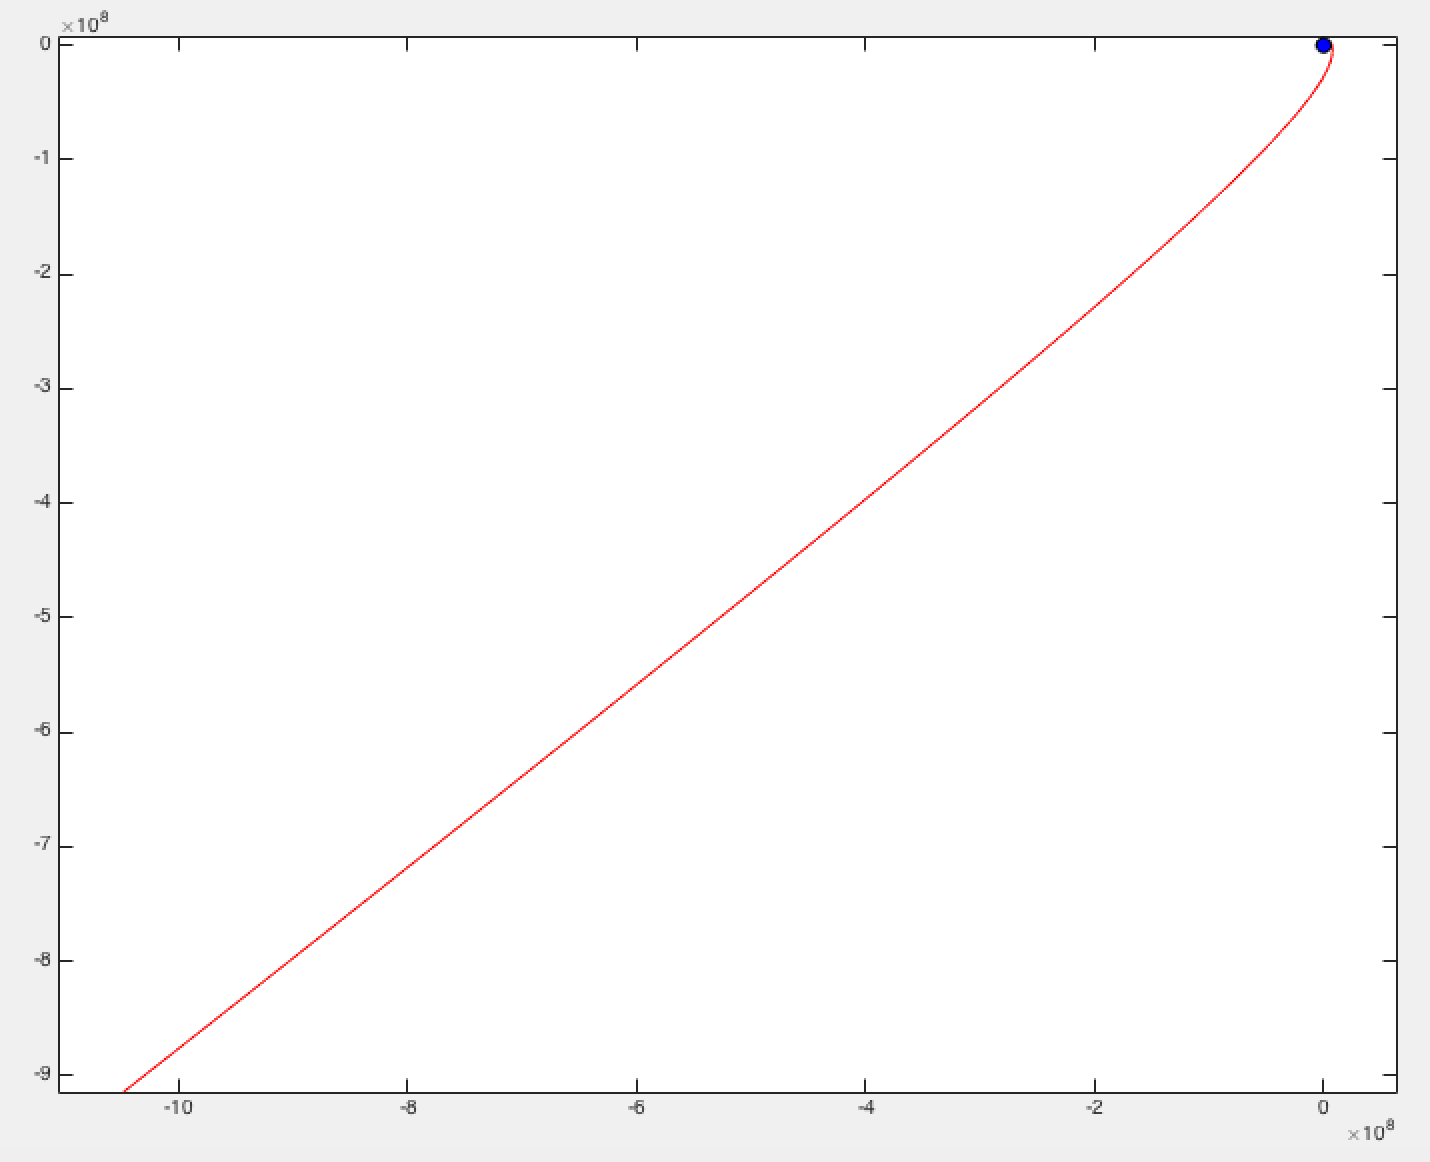
\includegraphics[width=0.5\textwidth]{../aufgabe1/screens/1b.png}
		\caption{Flucht des Satelliten von der Erdumlaufbahn}
	\end{figure}

\subsubsection{Geostationäre Bahn} 

Bei einer Starthöhe von $h_0 = 36000 km$ und einer Startgeschwindigkeit von $v0 = 3000 m/s$ ergibt sich eine genau ein Tag dauernde Umkreisung der Erde.
	
	\begin{figure}[H]
		\centering
		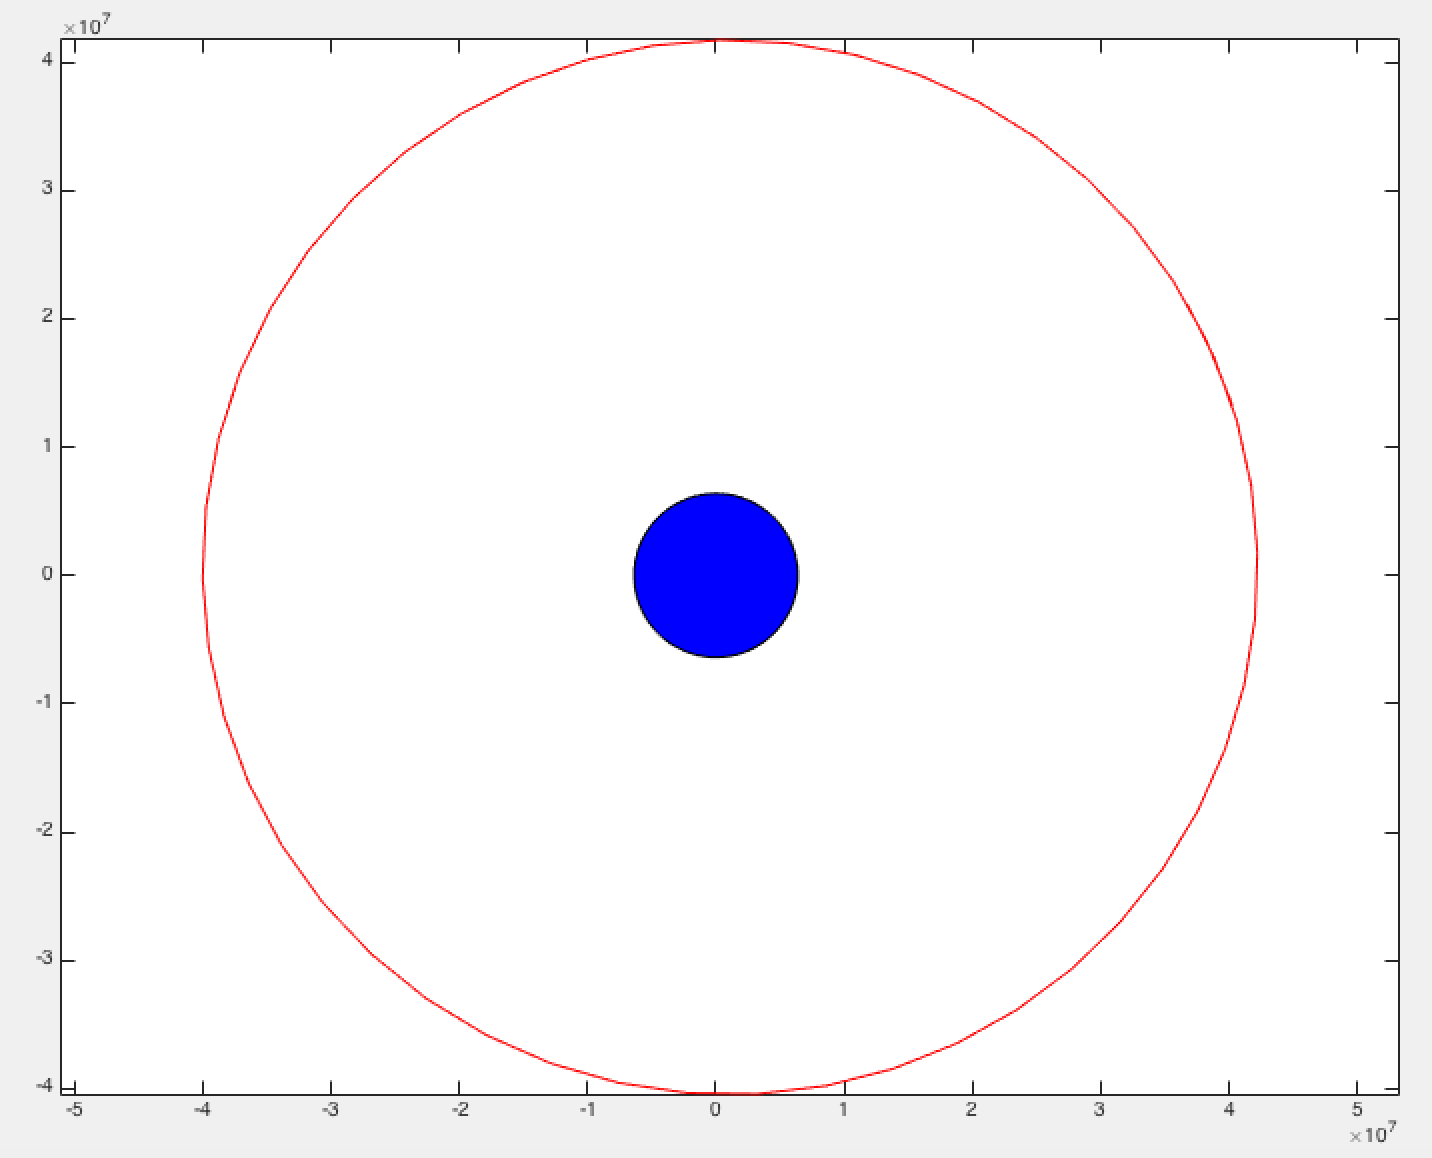
\includegraphics[width=0.5\textwidth]{../aufgabe1/screens/1c.png}
		\caption{Geostationäre Bahn}
	\end{figure}


\subsection{Mondumkreisung}

Die Schaltung ändert sich gegenüber der Erdumkreisung nicht.

	\begin{figure}[H]
		\centering
		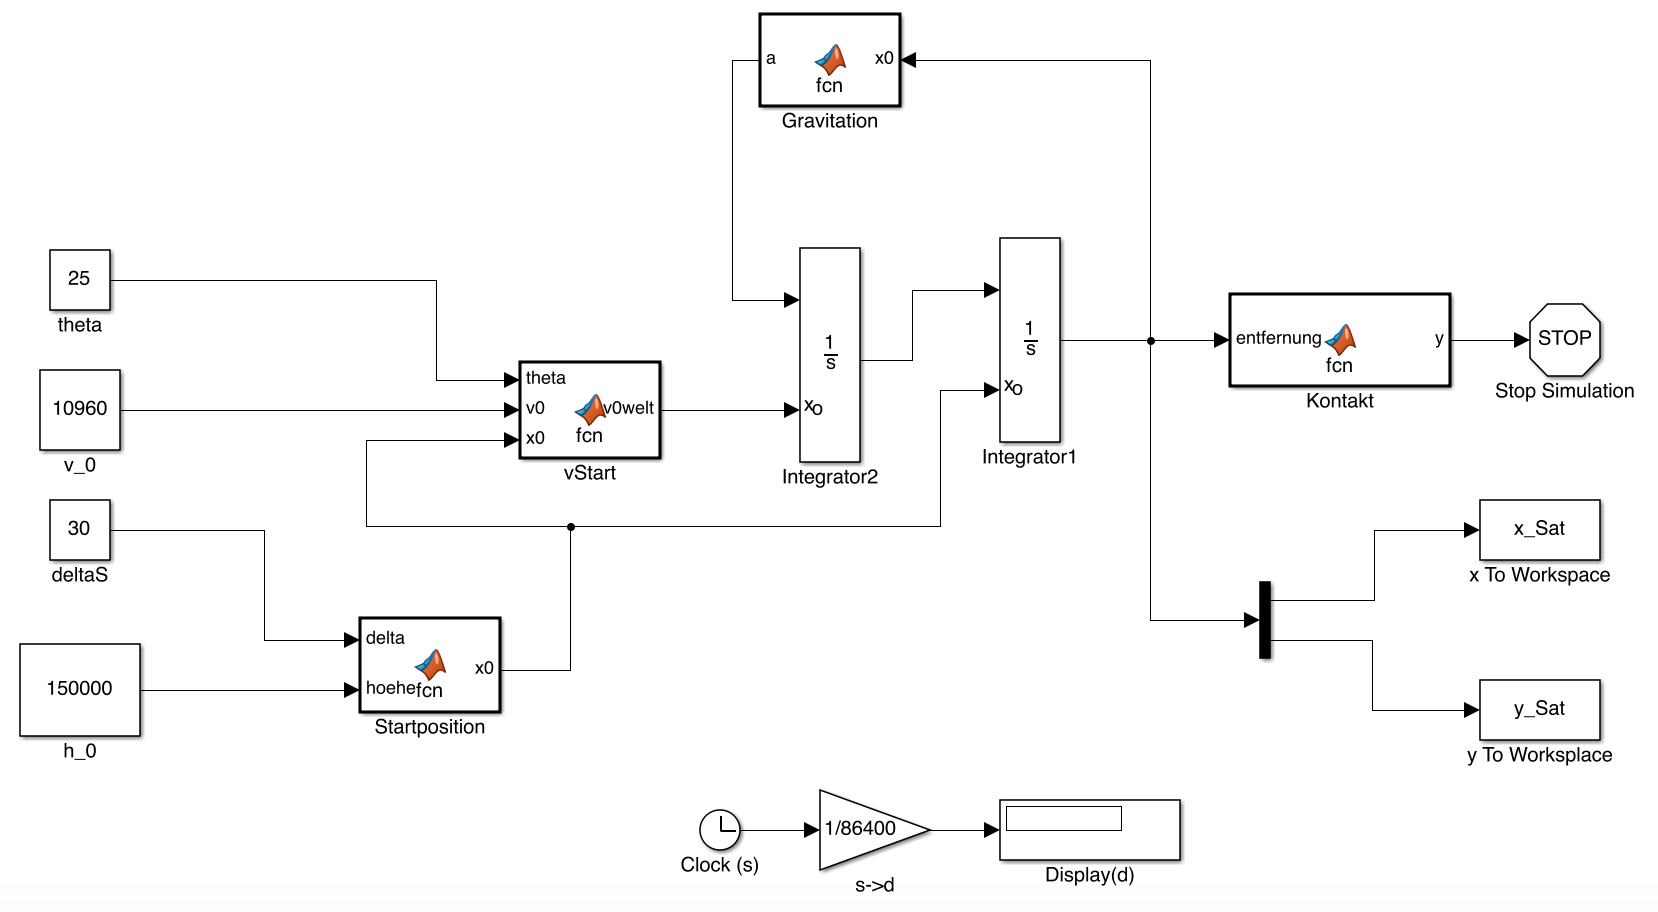
\includegraphics[width=1\textwidth]{../aufgabe12/screens/simulink_mond.png}
		\caption{Erd- und Mondumkreisung des Satelliten}
	\end{figure}

Die Gravitation ändert sich wie folgt:

\begin{align}
function \:  a = Gravitation(x_0)
\\G = 66.743 * 10^(-12); \nonumber % Gravitationskonstante
\\m_{Erde} = 5.9736 * 10^24; \nonumber% Masse der Erde
\\x_{Mond} = [0 ; -380000000] \nonumber% Position des Monds
\\m_{Mond} = 7.3480 * 10^22; \nonumber% Masse des Mondes
\\v_{Mond} =  x_0 - x_{Mond}; \nonumber% Vektor Sat richtung Mond
\\r_{Erde} = norm(x_0); \nonumber% Entfernung zur Erde
\\r_{Mond} = norm(v_{Mond}); \nonumber% Entfernung zum Mond
\\richtung_E = -x_0 / r_{Erde}; \nonumber% Einheitsvektor Erde-Satelit
\\richtung_M = -v_{Mond} / r_{Mond}; \nonumber% Einheitsvektor Mond-Satelit
\\a_{Mond} = richtungM * G * m_{Mond} / r_{Mond}^2 \nonumber
\\a = (richtung_E * G * m_{Erde} / r_{Erde}^2) + a_{Mond}; \nonumber% Gravitationsbeschl.
\end{align}

Bei einer Startgeschwindigkeit von $v0 = 10960 m / s$ und $\theta = 25^\circ$ ergibt sich eine achtförmige Umkreisung um Mond und Erde.

 	\begin{figure}[H]
 		\centering
 		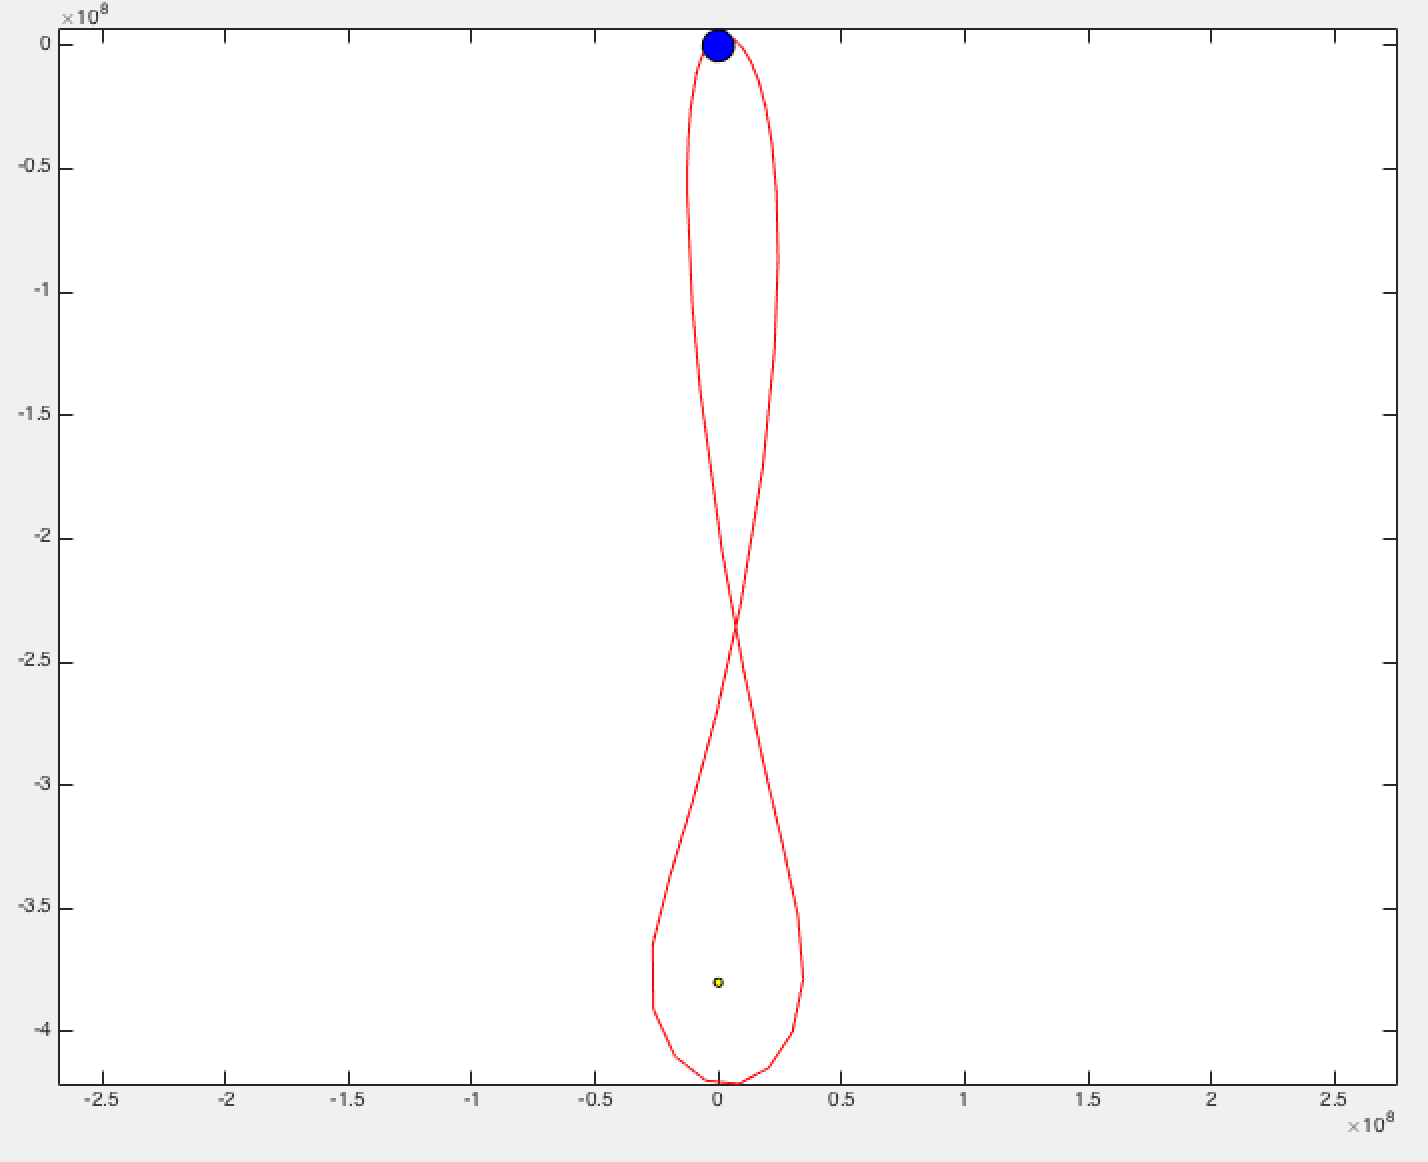
\includegraphics[width=0.5\textwidth]{../aufgabe12/screens/2.png}
 		\caption{Erdumkreisung des Satelliten}
 	\end{figure}

\section{Crazy Pendulum}

	\begin{figure}[H]
 		\centering
 		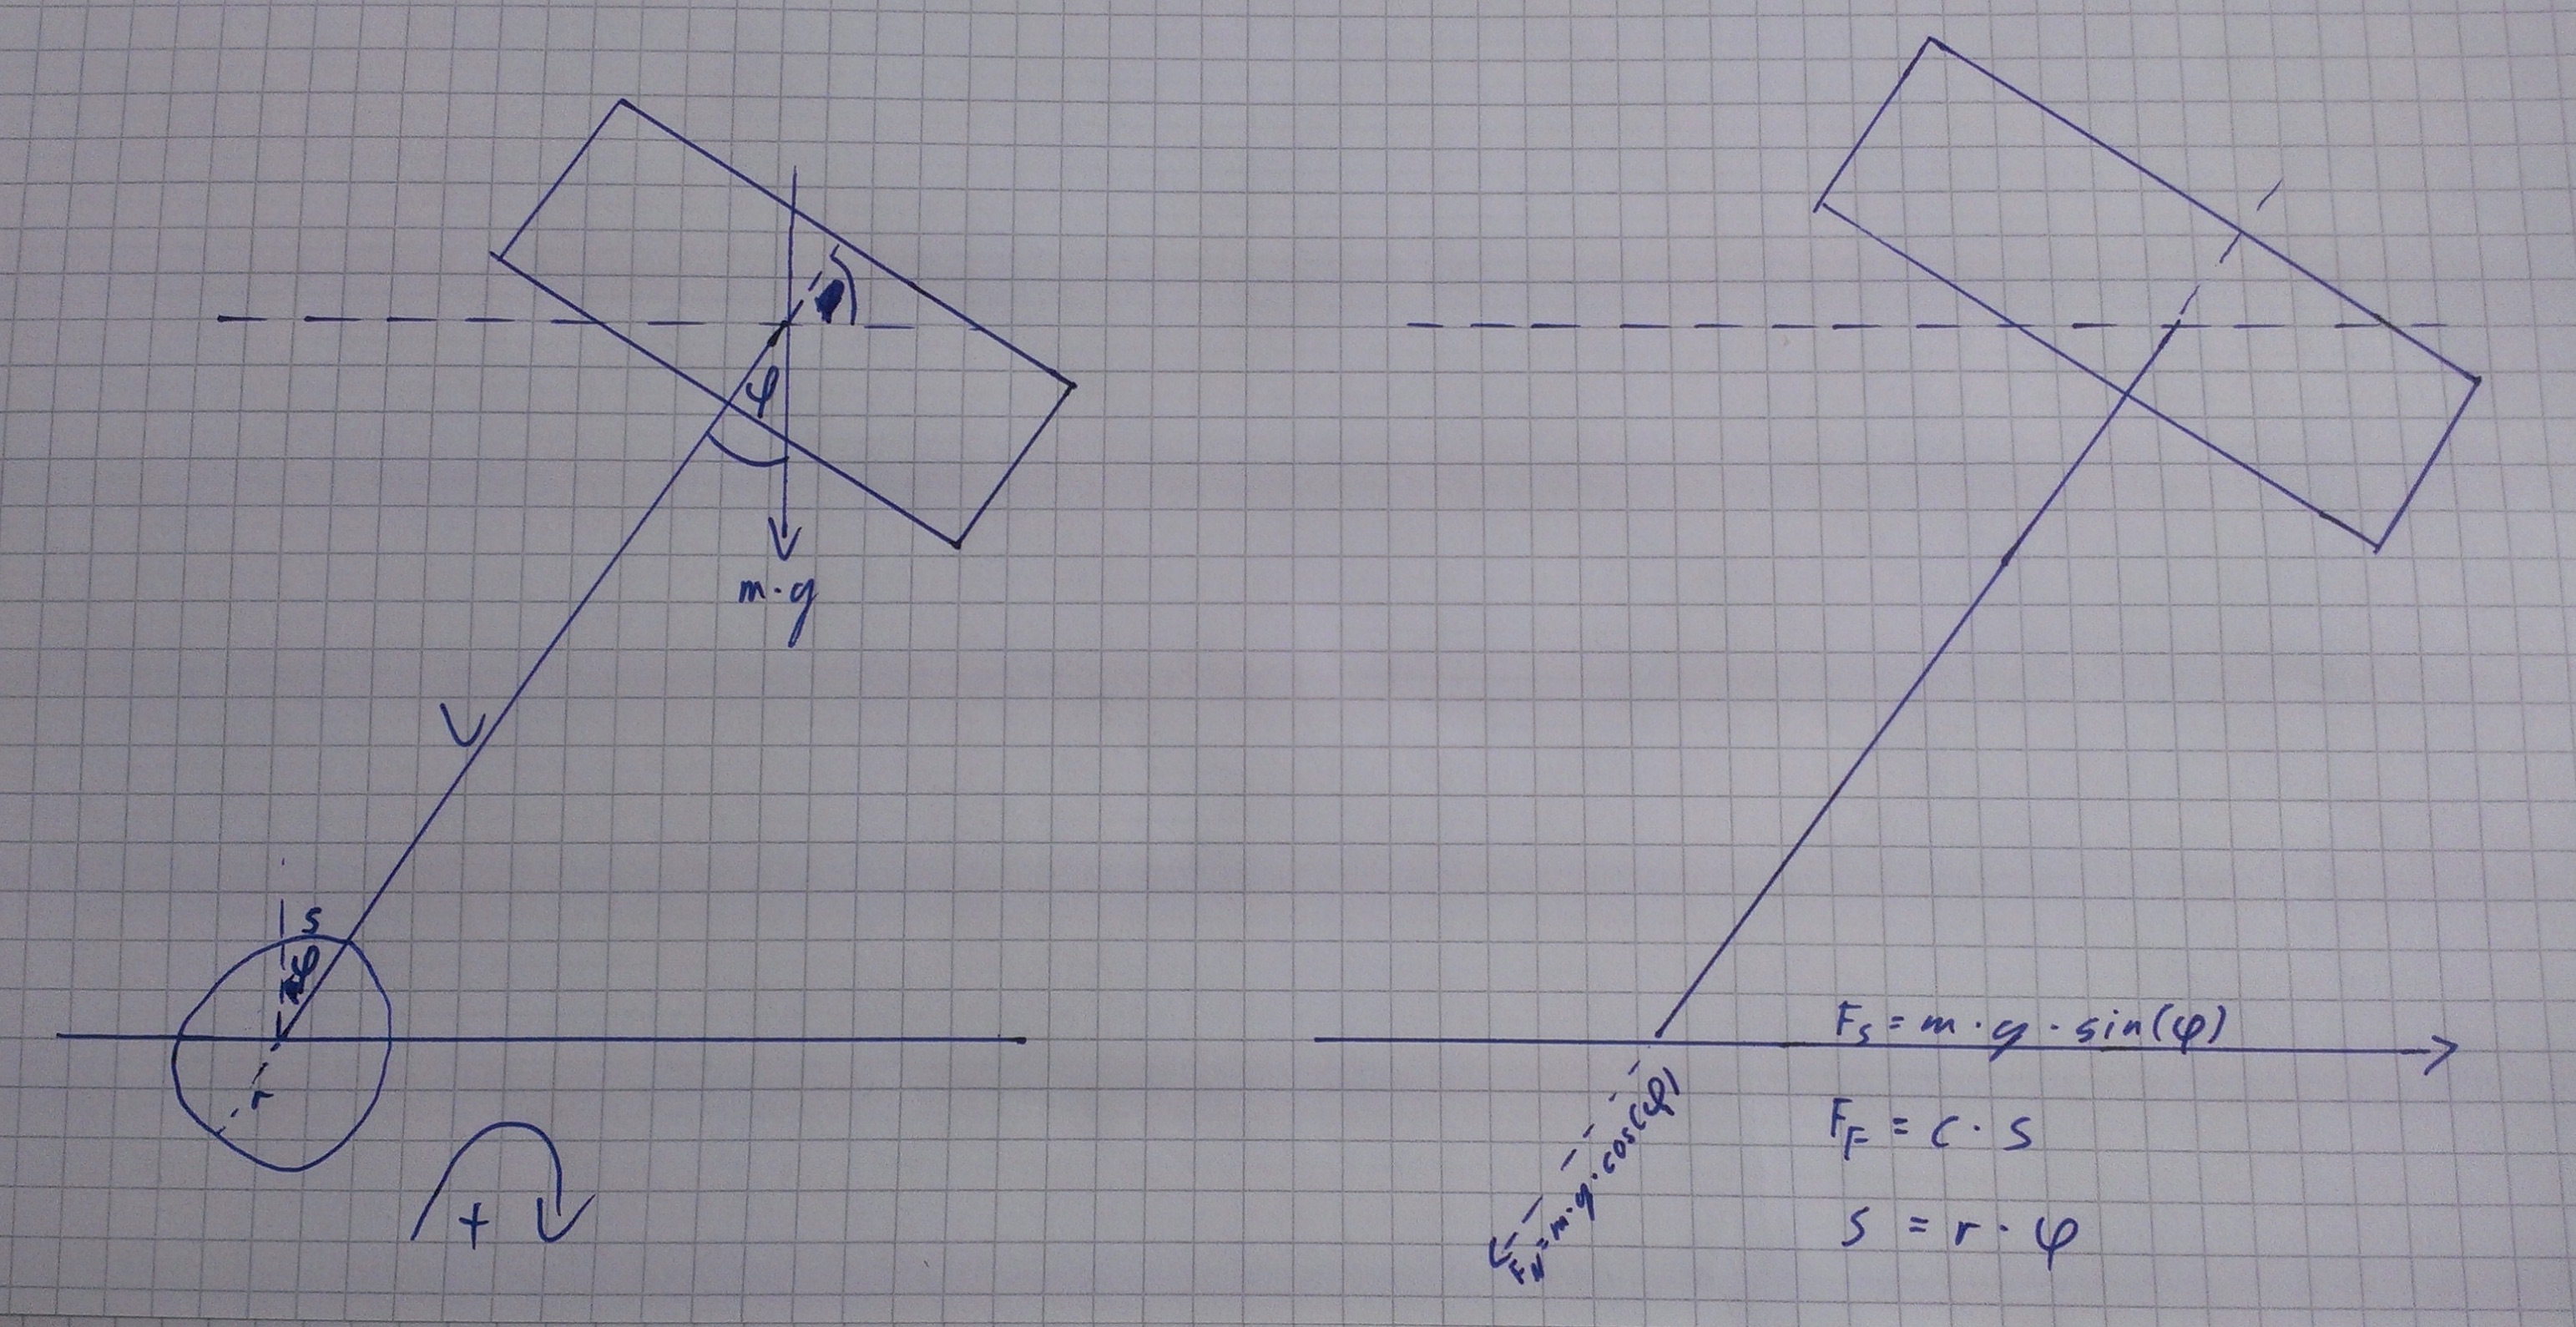
\includegraphics[width=1\textwidth]{../aufgabe2/Freikoerper.jpg}
 		\caption{Schaltbild Crazy Pendulum}
 	\end{figure}

 	\begin{figure}[H]
 		\centering
 		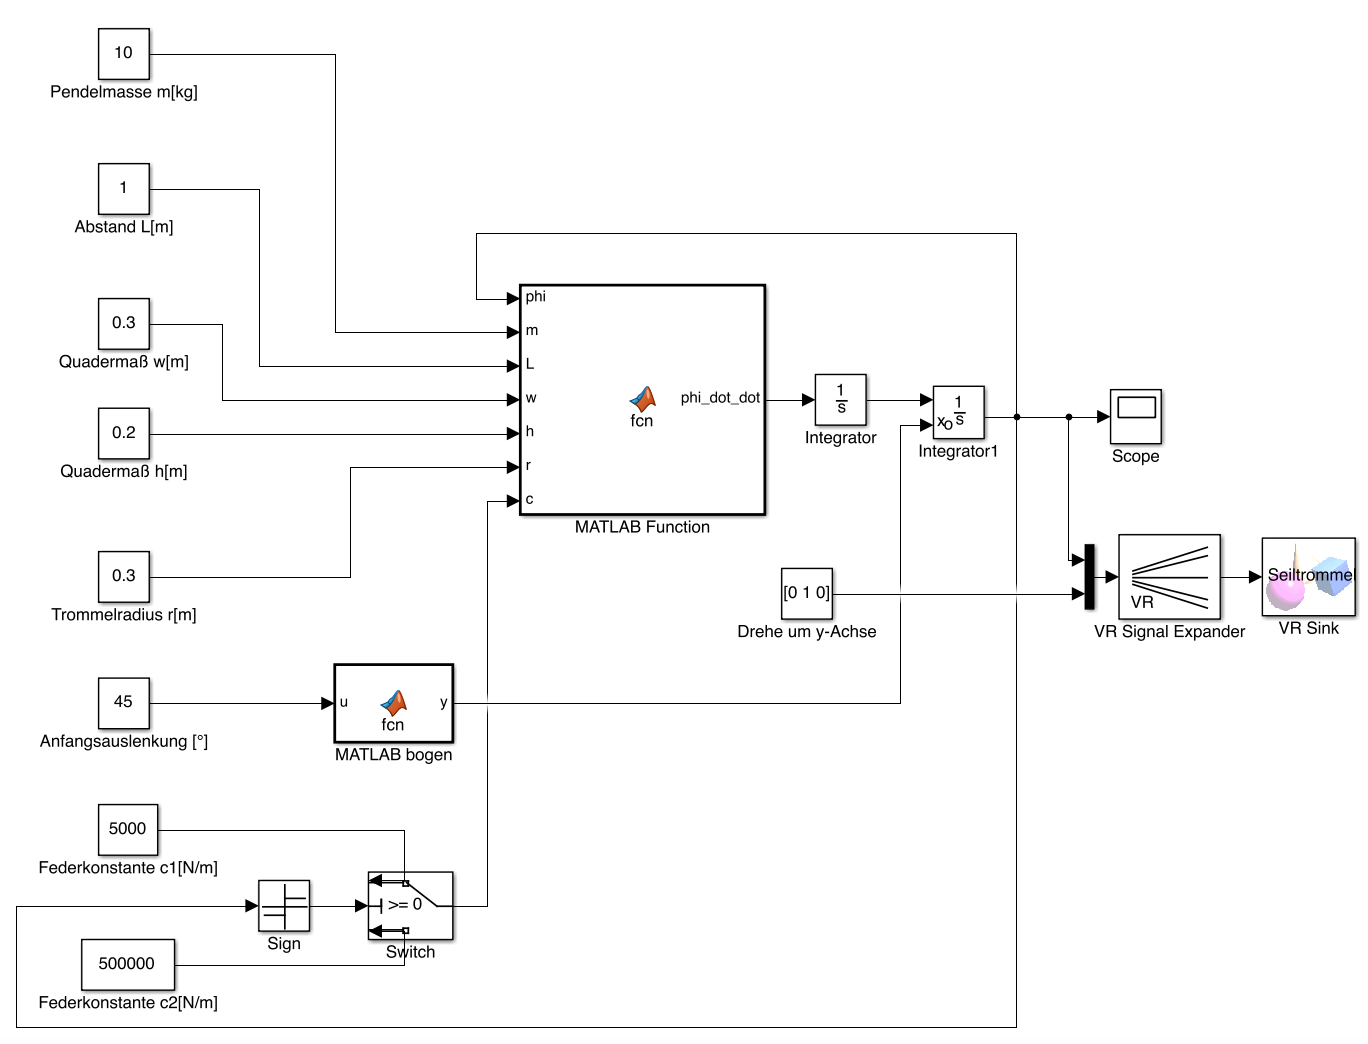
\includegraphics[width=1\textwidth]{../aufgabe2/simulink.png}
 		\caption{Schaltbild Crazy Pendulum}
 	\end{figure}
 	Die Winkelbeschleunigung ist wie folgt:
 	\begin{align}
 	function \: phi'' = fcn(phi, m, L, w, h, r, c)
 	\\g = 9.81; \nonumber
 	\\M_g = m * g * sin(phi)*(L+h/2);\nonumber
 	\\M_f = r * r * phi * c;\nonumber
 	\\J_s = (1/12 * m * (h^2) + (w^2));\nonumber
 	\\J_a = J_s + m * ((L+h/2)^2);\nonumber
 	\\phi'' = ( M_g - M_f ) / ( J_a );\nonumber
 	\end{align}
 	
 	Daraus ergibt sich eine Bewegung des Pendels:
 	 	\begin{figure}[H]
 	 		\centering
 	 		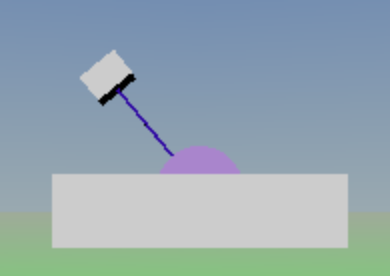
\includegraphics[width=0.5\textwidth]{../aufgabe2/pendel.png}
 	 		\caption{Schaltbild Crazy Pendulum}
 	 	\end{figure}
 	Die Winkelkurve ähnelt einem Sinus,zeigt jedoch die die Eigenschaften der Feder. Der Hochpunkt wird durch eine relativ geringe Steigung erreicht, die durch den weiche Feder bestimmt wird. Der Tiefpunkt wird durch die harte Feder mit einer höheren Steigung erreicht. 
 		\begin{figure}[H]
 	 		\centering
 	 		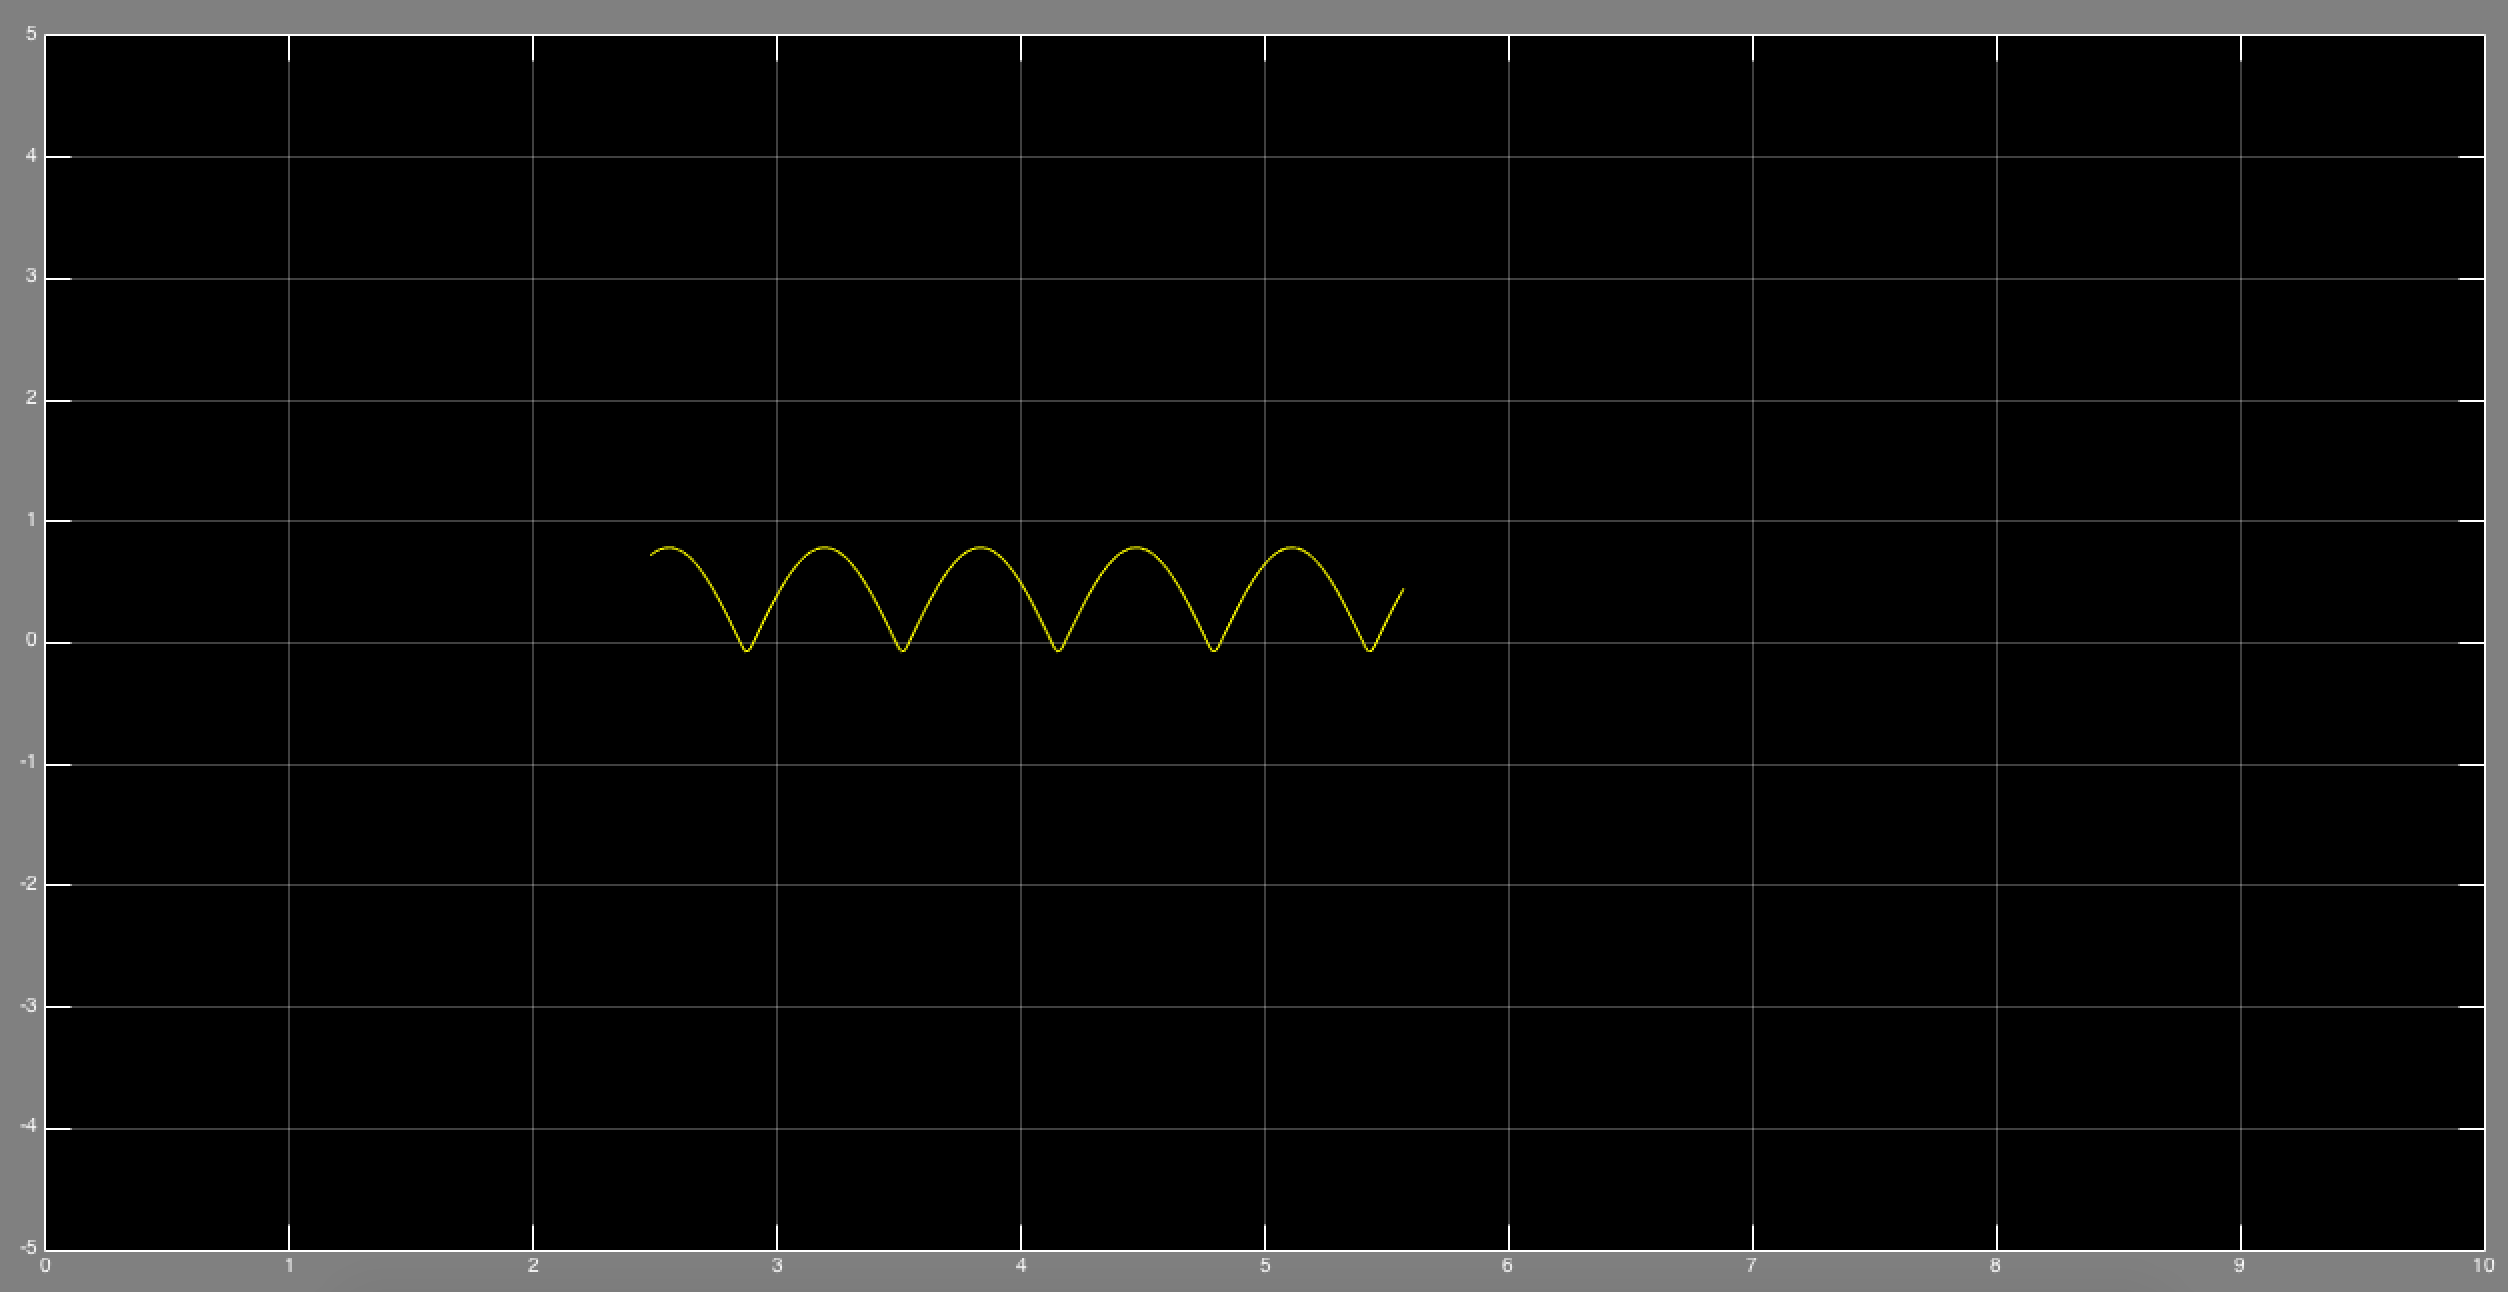
\includegraphics[width=1\textwidth]{../aufgabe2/phit.png}
 	 		\caption{$\phi(t)$}
 	 	\end{figure}

\section{Schwingungsgedämpfter Tisch}

\end{document}
